% !TeX root=../main.tex
\قسمت{مقدمه}
ایستگاه هواشناسی، مرکزی مجهز به تجهیزات و ابزارهایی برای اندازه گیری‌های جوی است که به ارائه اطلاعات برای پیش بینی و مطالعه آب و هوا می‌پردازد. اندازه گیری های انجام شده معمولا شامل دما، فشار هوا، رطوبت، سرعت باد، جهت باد و مقدار بارش است. مشاهدات دستی حداقل یک بار در روز انجام می شود، در حالی که اندازه گیری های خودکار حداقل یک بار در ساعت انجام می‌پذیرد.

ایستگاه های هواشناسی معمولی مجهز به ابزارهای زیر هستند \مرجع{wikipedia:Weather_station}:

\شروع{فقرات}
\فقره
رطوبت‌سنج برای اندازه گیری رطوبت
\فقره
فشارسنج برای اندازه گیری فشار جو
\فقره 
دماسنج برای اندازه گیری دمای هوا
\فقره
پیرانومتر برای اندازه گیری تشعشعات خورشیدی
\فقره
باران‌سنج برای اندازه گیری میزان بارش باران در طی یک دوره زمانی مشخص
\فقره
تجهیزاتی نظیر بادسنج، پرچم باد یا جوراب باد برای اندازه گیری سرعت و جهت باد
\پایان{فقرات}

ایستگاه های پیشرفته تر همچنین ممکن است شاخص فرابنفش، رطوبت برگ، رطوبت خاک، دمای خاک، دمای آب در حوضچه ها، دریاچه ها، نهرها یا رودخانه ها و گاهی داده های دیگر را اندازه گیری کنند. به جز دستگاه‌هایی که نیازمند تماس مستقیم با عناصر مورد اندازه گیری هستند (نظیر بادسنج)، دیگر سنسورها و دستگاه‌ها باید در محفظه‌ای به دور از تابش مستقیم خورشید و وزش باد قرار بگیرند.

ایستگاه‌های هواشناسی سینوپتیک 24 ساعته به صورت خودکار هر سه ساعت به سه ساعت پارامتر‌های جوی را پس از اندازه‌گیری و جمع‌آوری از طریق شبکه‌های مخابراتی منتقل می‌کنند. به طور مشابه ایستگاه‌هایی با نام متار این کار را هر  یک ساعت انجام‌ می‌دهند. وظیفه این ایستگاه‌ها جمع‌آوری اطلاعات جوی از محدوده‌هایی وسیع و مخابره به ایستگاه‌های اصلی به منظور اطلاع از وضعیت حال و گذشته و پیش بینی شرایط آب و هوایی مناطق در آینده است. 

هدف این پروژه پیاده سازی نوعی ایستگاه هواشناسی سینوپتیک است که با تجهیزات ارزان و کم‌مصرف دیجیتالی پارامتر‌های جوی لازم را جمع آوری و به صورت بی‌سیم به ایستگاهی جهت ثبت و نمایش مخابره می‌کند. در این پروژه از میکروکنترلرهای \متن‌لاتین{ARM} سری \متن‌لاتین{STM32F10X} به عنوان هسته اصلی پردازش در هر دو سمت سنسور و ایستگاه و از ماژول لورا (\متن‌لاتین{LoRa}) با چیپ \متن‌لاتین{SX1278} به منظور برقراری ارتباط بی‌سیم استفاده می‌شود.

\قسمت{اجزای سیستم}

این سیستم به دو دستگاه اصلی تقسیم می‌شود، یک دستگاه جهت جمع آوری اطلاعات جوی برروی یک میله در ارتفاع 10 متری سطح زمین قرار می‌گیرد و اطلاعات جوی نظیر دما، رطوبت، فشار، شدت نور، سرعت و جهت باد را از سنسور‌های مربوطه جمع آوری کرده و به صورت بی‌سیم به دستگاه دیگر، که در ایستگاه اصلی قرار دارد، مخابره می‌کند؛ سپس اطلاعات دریافت شده در دستگاه دوم جهت ثبت و ذخیره به رایانه منتقل می‌شود. در اینجا به دستگاه اول که وظیفه جمع آوری اطلاعات جوی را دارد سنسور و دستگاه دوم که وظیفه دریافت اطلاعات مخابره شده و انتقال به رایانه را دارد ایستگاه می‌گوییم. بلوک دیاگرام کلی این سیستم و نحوه ارتباط بخش‌های مختلف با یکدیگر در شکل \رجوع{fig:systemDesign} آمده است.

\begin{figure}[!h]
	\centering
	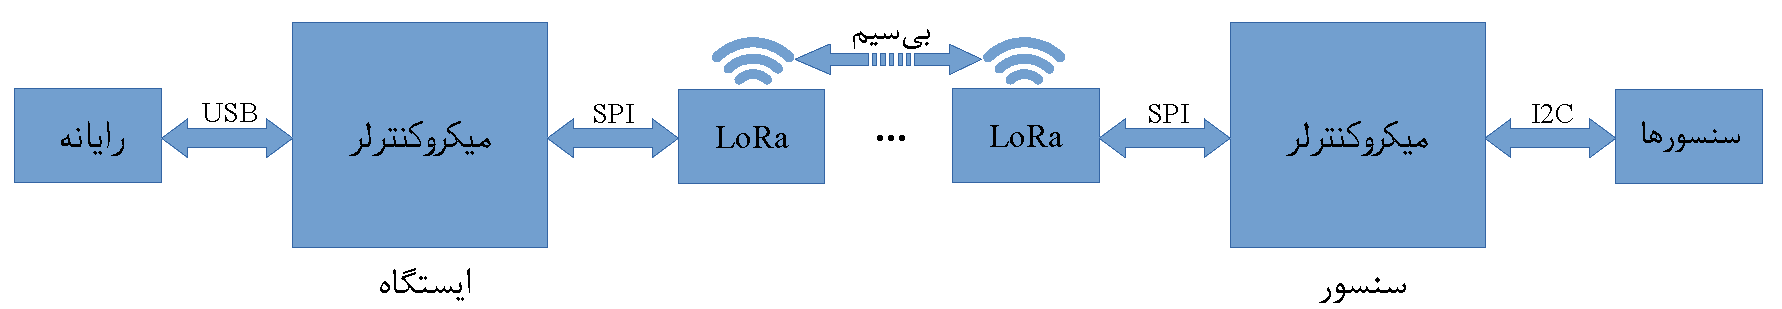
\includegraphics[width=\linewidth]{Assets/system design.pdf}
	\caption{بلوک دیاگرام اجزای سیستم و نحوه ارتباط اجزای مختلف با یکدیگر.}
	\label{fig:systemDesign}
\end{figure}

\زیرقسمت{میکروکنترلر}

هسته اصلی پردازش در هر دو سمت ایستگاه و سنسور میکروکنترلر \متن‌لاتین{STM32f103CBT6} انتخاب شده است که با توجه به موجود بودن در بازار ایران و دارا بودن 2 عدد \متن‌لاتین{I2c}، 2 عدد \متن‌لاتین{SPI}، اینترفیس \متن‌لاتین{USB} و 3 عدد تایمر 16 بیتی نیاز به حداقل 1 عدد \متن‌لاتین{I2c} (در سمت سنسور)، 1 عدد \متن‌لاتین{SPI} (در هر دو سمت)، اینترفیس \متن‌لاتین{USB} (در سمت ایستگاه)  و 1 عدد تایمر (در سمت سنسور) را برآورده می‌کند. همچنین حالت \متن‌لاتین{Sleep} و واحد \متن‌لاتین{RTC} موجود در این میکروکنترلر‌ها به کاهش مصرف انرژی در وقفه‌های سه ساعته کمک می‌کند؛ به طوری که استفاده از سیستم باتری و پنل خورشیدی را ممکن می‌سازد.

\زیرقسمت{ارتباط بی‌سیم}



\زیرقسمت{سنسورها}

\زیرزیرقسمت{سنسور \متن‌لاتین{BMP180}}

\زیرزیرقسمت{سنسور \متن‌لاتین{MAX44009}}

\زیرزیرقسمت{سنسور \متن‌لاتین{QMC5883L}}

\زیرزیرقسمت{سنسور \متن‌لاتین{AHT10}}

\زیرزیرقسمت{سنجش شدت و جهت باد}

در سنجش شدت و جهت باد در روش مکانیکی از دو ابزار به صورت مستقل (در برخی موارد این دو ابزار در قالب یک دستگاه در کنار هم قرار میگیرند)، یک ابزار برای سنجش شدت و ابزاری دیگر برای تعیین جهت، امورد استفاده قرار می‌گیرد. هر دو دستگاه دارای قطعات متحرک اند و یکی با داشتن پره‌هایی شبیه به دم هلی کوپتر با وزرش باد در جهت وزش قرار میگیرد و دیگری دارای پره‌هایی است که با وزش باد پره‌ها همانند پره‌های توربین به حدکت در می‌آید که با توجه به سرعت چرخش پره‌ها سرعت باد قابل اندازه‌ گیری است. در اندازه‌گیری‌های این دستگاه‌ها محدودیت‌هایی وجود دارد و اغلب این نوع ابزارها در وزش باد ملایم عملکرد صحیحی از خود نشان نمی‌دهند. همچنین در اندازه گیری زاویه وزش ممکن اند محدود به زوایای خاصی باشند. 

در روش اندازه‌گیری شدت و جهت باد با آلتراسونیک اندازه‌گیری‌ها می‌تواند در قالب تنها یک دستگاه ،بدون قطعات متحرک و با دقتی بالاتر انجام پذیرد. در این روش 2 فرستنده و گیرنده آلتراسونیک همان طور که در شکل \رجوع{fig:oneAxisUltrasonic} نشان داده شده است روبروی یکدیگر در فاصله‌ مشخص $d$ قرار داده می‌شوند.

\begin{figure}[!h]
	\centering
	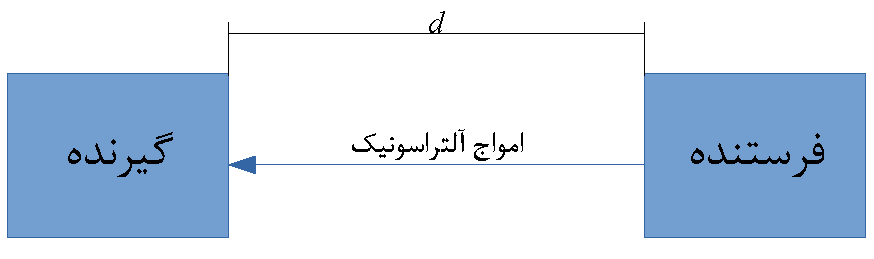
\includegraphics[width=0.6\linewidth]{Assets/ultrasonic one axis.pdf}
	\caption{نحوه قرار گیری فرستنده و گیرنده آلتراسونیک.}
	\label{fig:oneAxisUltrasonic}
\end{figure}

فرستنده امواج صوتی با فرکانس 40 کیلو هرتز تولید می‌کند. فاصله زمانی بین ارسال امواج صوتی از فرستنده و دریافت این امواج در گیرنده اندازه‌گیری می‌شود. با توجه به رابطه \رجوع{eq:speed} سرعت $v$ با داشتن با داشتن فاصله $d$ و زمان تاخیر بین ارسال موج صوتی در فرستنده و دریافت آن در گیرنده  $t$ قابل اندازه گیری است.
\begin{equation}\label{eq:speed}
	v = \frac{d}{t}
\end{equation}

سرعت $v$ بدست آمده از این رابطه مطابق رابطه \رجوع{eq:expandSpeed} متشکل از سرعت صوت $v_s$ و سرعت باد $v_{wx}$  است \مرجع{7988049}.
\begin{equation}\label{eq:expandSpeed}
	v = v_s + v_{wx}
\end{equation}

در صورتی که وزش باد در جهت موافق حرکت امواج صوتی باشد زمان تاخیر در دریافت امواج نسبت به حالی که باد نوزد کمتر شده و در نتیجه سرعت $v$ نسبت به حالتی که باد نوزد افزایش می‌یابد (یعنی علامت $v_{wx}$ مثبت بوده و $v = v_s+v_{wx}$). در صورتی که وزش باد در خلاف جهت حرکت امواج صوتی باشد زمان تاخیر در دریافت امواج نسبت به حالتی که باد نوزد بیشتر شده و در نتیجه سرعت $v$ کاهش می‌یابد (یعنی علامت $v_{wx}$ منفی بوده و $v = v_s-v_{wx}$). با داشتن سرعت صوت $v_s$، فاصله $d$ و محاسبه زمان $t$ میتوان با توجه به معادلات \رجوع{eq:speed} و \رجوع{eq:expandSpeed} سرعت باد $v_{wx}$ و جهت باد (علامت سرعت $v_{wx}$) روی یک محور مطابق رابطه \رجوع{eq:speedWindX} بدست آورد. 

\begin{equation}\label{eq:speedWindX}
	v_{wx} = \frac{d}{t} - v_s
\end{equation}

به منظور سنجش شدت و جهت باد در دو بعد می‌توان دو فرستنده و گیرنده دیگر برروی محوری عمود بر محور متصل کننده فرستده و گیرنده فعلی قرار داد و با محاسبه دو بردار سرعت، بردار سرعت برآیند را بدست آورد.

\begin{figure}[!h]
	\begin{subfigure}[b]{0.5\textwidth}
		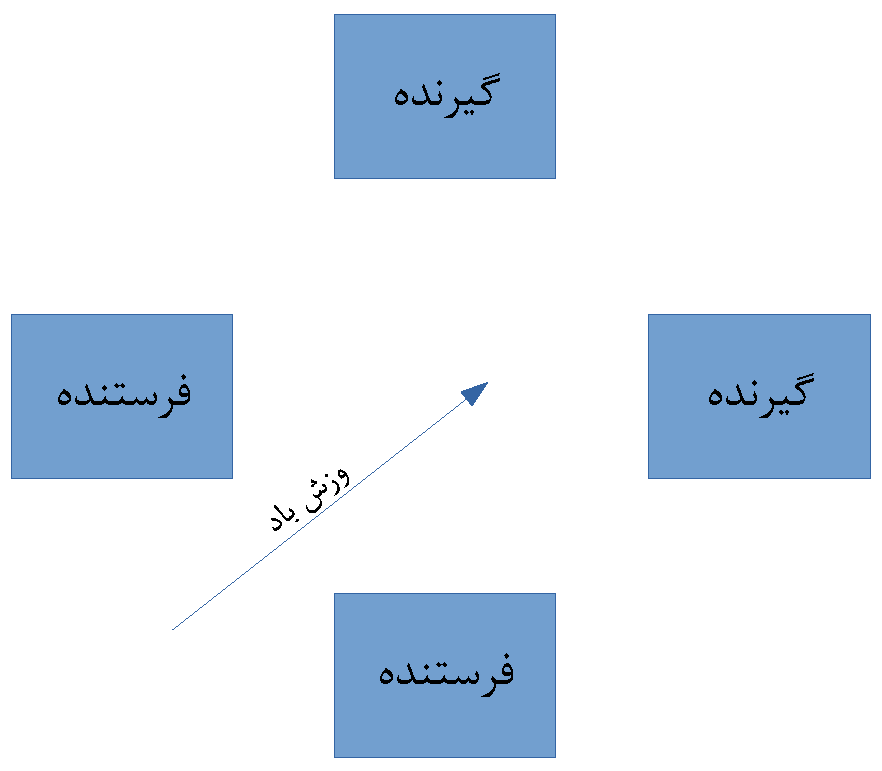
\includegraphics[width=\linewidth]{Assets/ultrasonic 2d.pdf}
		\caption{}
		\label{fig:2dUltrasonic}
	\end{subfigure}
	\begin{subfigure}[b]{0.5\textwidth}
		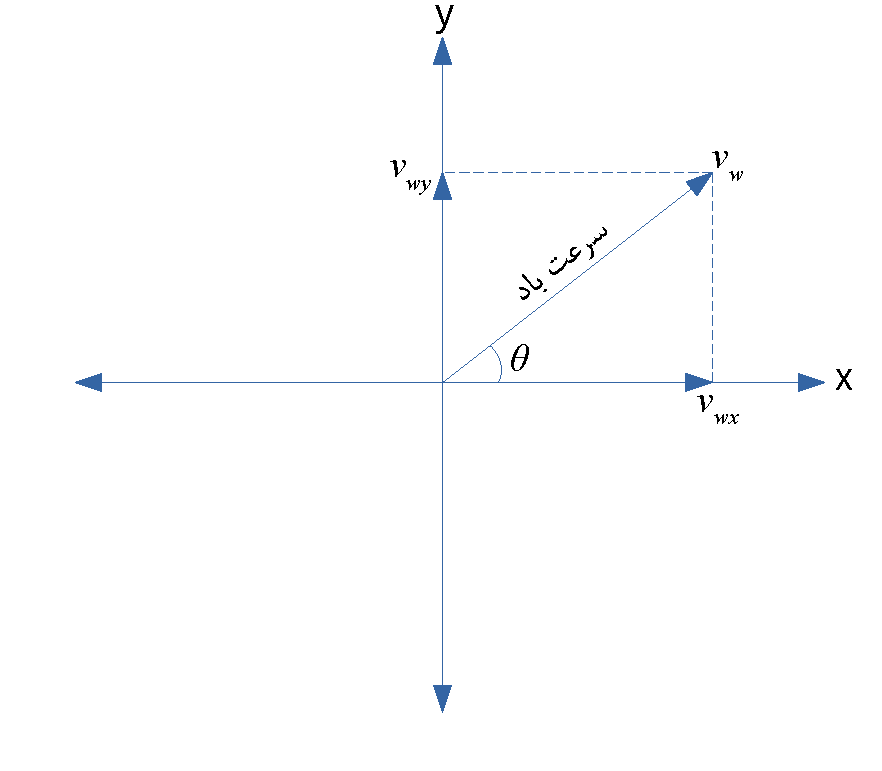
\includegraphics[width=\linewidth]{Assets/ultrasonic 2d axis.pdf}
		\caption{}
		\label{fig:2dUltrasonicAxis}
	\end{subfigure}
	\caption{نحوه قرار گیری فرستنده و گیرنده آلتراسونیک دو محوره و نمودار متناظر با آن‌ها.}
\end{figure}

اگر نحوه قرار گیری فرستنده و گیرنده‌ها مطابق شکل \رجوع{fig:2dUltrasonic} باشد در این صورت صفحه مختصات متناظر با آن مطابق شکل \رجوع{fig:2dUltrasonicAxis} خواهد بود. اندازه $v_w$ و زاویه $\theta$ بردار سرعت باد از طریق روابط \رجوع{eq:windSpeed} بدست می‌آیند.

\begin{equation}\label{eq:windSpeed}
	\begin{split}
		v_w = \sqrt{v_{wx}^2 + v_{wy}^2}\\
		\theta = \tan^{-1}{\left( \frac{v_{wy}}{v_{wx}}\right)}
	\end{split}	
\end{equation}

\begin{table}[!t]
	\centering
	\caption{ضرایت  محاسبه سرعت صوت (فرمول \رجوع{eq:soundSpeed})}
	\label{tb:speedOfSoundcoefficients}
	\begin{tabular}{cc}
		\hline \hline
		 ضرایب & \\
		\hline
		$a_{0}$ & $331.5024$ \\
		$a_{1}$ & $0.603055$ \\
		$a_{2}$ & $-0.000528$ \\
		$a_{3}$ & $51.471935$ \\
		$a_{4}$ & $0.1495874$ \\
		$a_{5}$ & $-0.000782$ \\
		$a_{6}$ & $-1.82 \times 10^{-7}$ \\
		$a_{7}$ & $3.73 \times 10^{-8}$ \\
		$a_{8}$ & $-2.93 \times 10^{-10}$ \\
		$a_{9}$ & $-85.20931$ \\
		$a_{10}$ & $-0.228525$ \\
		$a_{11}$ & $5.91 \times 10^{-5}$ \\
		$a_{12}$ & $-2.835149$ \\
		$a_{13}$ & $-2.15 \times 10^{-13}$ \\
		$a_{14}$ & $29.179762$ \\
		$a_{15}$ & $0.000486$ \\
		\hline
	\end{tabular}
\end{table}

سرعت صوت $v_s$ به عنوان تابعی از دما، فشار و کسر مولی رطوب و کربن دی اکسید، با استفاده از رابطه \رجوع{eq:soundSpeed} قابل محاسبه است \مرجع{cramer1993variation}. ثوابت$a_1$ تا $a_{15}$ در جدول \رجوع{tb:speedOfSoundcoefficients} آمده اند.

\begin{equation}\label{eq:soundSpeed}
	\begin{aligned}
		v_s\left(\tau, p, x_w, x_{c}\right)=& a_{0}+a_{1} \tau+a_{2} \tau^{2}+\left(a_{3}+a_{4} \tau+a_{5} \tau^{2}\right) x_{w} \\
		&+\left(a_{6}+a_{7} \tau+a_{8} \tau^{2}\right) p+\left(a_{9}+a_{10} \tau+a_{11} \tau^{2}\right) x_{c} \\
		&+a_{12} x_{w}^{2}+a_{13} p^{2}+a_{14} x_{c}^{2}+a_{15} x_w p x_c
	\end{aligned}
\end{equation}

که $\tau$ دمای هوا (برحسب درجه سلسیوس)، $p$ فشار هوا (بر حسب پاسکال)، $x_w$ کسر مولی بخار آب در هوا و $x_c$ کسر مولی کربن دی‌اکسید در هوا است. $x_c$ را ثابت و برابر $400 \times 10^{-6}$ در نظر می‌گیریم. کسر مولی بخار آب در هوا $x_w$ از رابطه \رجوع{eq:x_w} بدست می‌آید \مرجع{rasmussen1997calculation}. 

\begin{equation}\label{eq:x_w}
	x_w=\frac{h f p_{sv}}{100 p}
\end{equation}

که $h$ درصد رطوب هوا، $p_{sv}$ فشار اشباع بخار آب در هوا و $f$ ضریب تقویت است و از طریق روابط 
\رجوع{eq:f} و \رجوع{eq:p_sv} محاسبه می‌شوند \مرجع{davis1992equation}.

\begin{equation}\label{eq:f}
	f=1.00062+3.14 \times 10^{-8} p+5.6 \times 10^{-7} \tau^{2}
\end{equation}
\begin{equation}\label{eq:p_sv}
	\begin{aligned}
		p_{s v}=& \exp \left(1.2811805 \times 10^{-5} T^{2}-1.9509874 \times 10^{-2} T\right.\\
		&\left.+34.04926034-6.3536311 \times 10^{3} / T\right)
	\end{aligned}
\end{equation}

که در این روابط $T$ دمای محیط بر حسب کلوین است، یعنی:
\begin{equation}
	T = \tau + 273.15
\end{equation}



